\begin{figure}
	\centering
	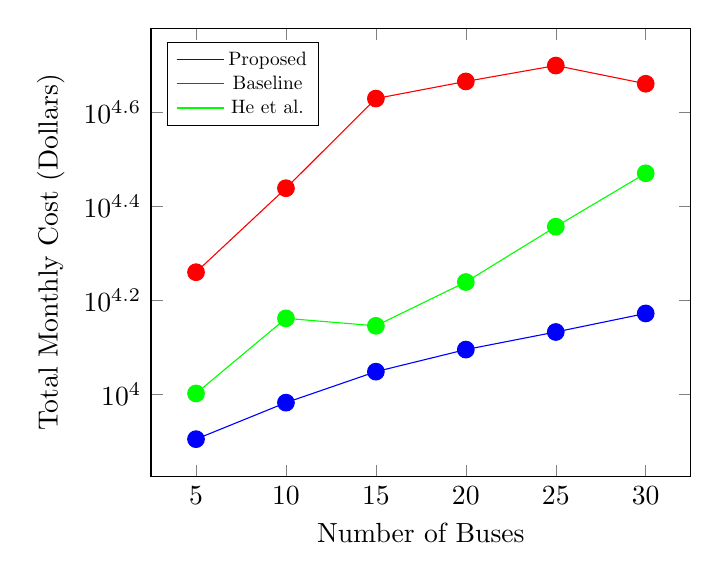
\begin{tikzpicture}
		\begin{axis}[xlabel=Number of Buses, ymode=log, ylabel=Total Monthly Cost (Dollars), legend pos=north west, legend style={nodes={scale=0.7}}]
			\addplot[blue] coordinates {
				(5,  8021.04 )
				(10, 9593.22 )
				(15, 11168.10)
				(20, 12445.52)
				(25, 13566.28)
				(30, 14857.82)}; 
			\addplot[red] coordinates{
				(5,  18190.02)
				(10, 27455.96)
				(15, 42618.54)
				(20, 46349.84)
				(25, 50101.33)
				(30, 45824.02)}; 
			\addplot[green] coordinates{
				(5,  10035.42)
				(10, 14505.31)
				(15, 13983.69)
				(20, 17333.25)
				(25, 22734.91)
				(30, 29543.78)
				};
			\addplot[blue, only marks, mark size=3pt] coordinates {
				(5,  8021.04 )
				(10, 9593.22 )
				(15, 11168.10)
				(20, 12445.52)
				(25, 13566.28)
				(30, 14857.82)}; 
			\addplot[red, only marks, mark size=3pt] coordinates{
				(5,  18190.02)
				(10, 27455.96)
				(15, 42618.54)
				(20, 46349.84)
				(25, 50101.33)
				(30, 45824.02)};
			\addplot[green, only marks, mark size=3pt] coordinates{
				(5,  10035.42)
				(10, 14505.31)
				(15, 13983.69)
				(20, 17333.25)
				(25, 22734.91)
				(30, 29543.78)
				};
			\legend{Proposed, Baseline, He et al.}
		\end{axis}
	\end{tikzpicture}
	\caption{Monthly Cost with 5 Chargers}
	\label{fig:scalabilityCost}
\end{figure}


